\documentclass[tikz,border=8pt]{standalone}
\usepackage{tikz}
\usetikzlibrary{arrows.meta,calc}

\definecolor{primary}{HTML}{143264}
\definecolor{secondary}{HTML}{8C281E}
\definecolor{tealcol}{HTML}{117A65}
\definecolor{orangecol}{HTML}{C77C02}
\definecolor{greycol}{HTML}{505A64}

\begin{document}
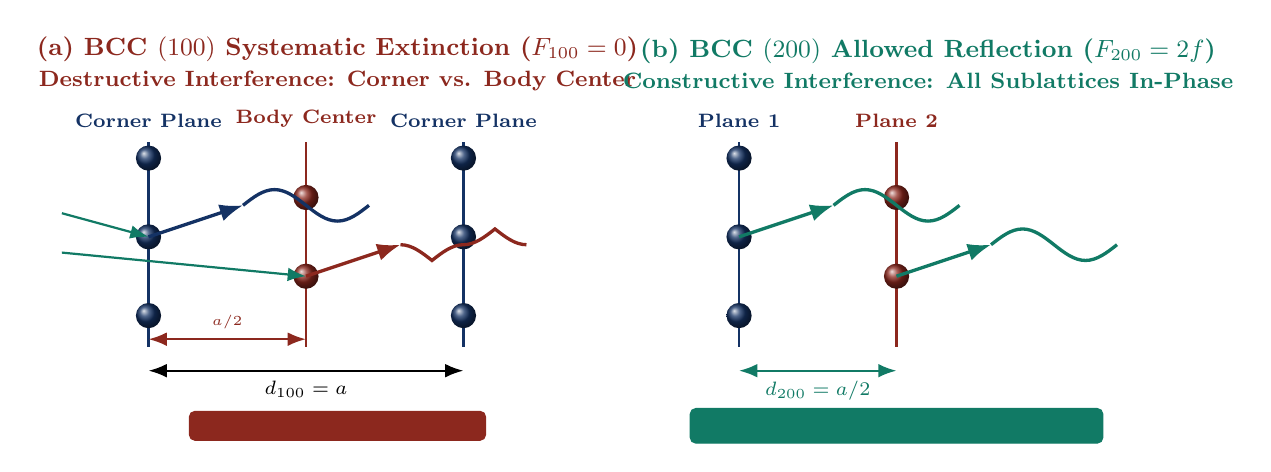
\begin{tikzpicture}[>=Latex]

  % Panel (a): Destructive Interference in BCC (100)
  \begin{scope}[shift={(0,0)}]
    \node[align=center, font=\bfseries\small, text=secondary] at (3.2, 4.2) 
      {(a) BCC $(100)$ Systematic Extinction ($F_{100}=0$)\\ \footnotesize Destructive Interference: Corner vs. Body Center};

    % Corner atom plane (x = 0)
    \draw[thick, primary] (0.8, 3.2) -- (0.8, 0.6);
    \foreach \y in {1.0, 2.0, 3.0} {
      \shade[ball color=primary] (0.8, \y) circle (0.16);
    }
    \node[above=2pt, font=\scriptsize\bfseries, primary] at (0.8, 3.2) {Corner Plane};

    % Body center atom plane (x = a/2)
    \draw[thick, secondary] (2.8, 3.2) -- (2.8, 0.6);
    \foreach \y in {1.5, 2.5} {
      \shade[ball color=secondary] (2.8, \y) circle (0.16);
    }
    \node[above=2pt, font=\scriptsize\bfseries, secondary] at (2.8, 3.2) {Body Center};

    % Next corner atom plane (x = a)
    \draw[thick, primary] (4.8, 3.2) -- (4.8, 0.6);
    \foreach \y in {1.0, 2.0, 3.0} {
      \shade[ball color=primary] (4.8, \y) circle (0.16);
    }
    \node[above=2pt, font=\scriptsize\bfseries, primary] at (4.8, 3.2) {Corner Plane};

    % Spacing d_100 = a
    \draw[<->, thick] (0.8, 0.3) -- (4.8, 0.3) node[midway, below, font=\scriptsize\bfseries] {$d_{100} = a$};
    \draw[<->, thick, secondary] (0.8, 0.7) -- (2.8, 0.7) node[midway, above, font=\tiny\bfseries] {$a/2$};

    % Incident waves
    \draw[->, thick, tealcol] (-0.3, 2.3) -- (0.8, 2.0);
    \draw[->, thick, tealcol] (-0.3, 1.8) -- (2.8, 1.5);

    % Reflected waves showing out-of-phase condition
    \draw[->, very thick, primary] (0.8, 2.0) -- (2.0, 2.4);
    \draw[very thick, primary] (2.0, 2.4) sin (2.4, 2.6) cos (2.8, 2.4) sin (3.2, 2.2) cos (3.6, 2.4);
    
    \draw[->, very thick, secondary] (2.8, 1.5) -- (4.0, 1.9);
    \draw[very thick, secondary] (4.0, 1.9) cos (4.4, 1.7) sin (4.8, 1.9) cos (5.2, 2.1) sin (5.6, 1.9);

    \node[draw=secondary!60, fill=secondary!10, rounded corners=2pt, inner sep=3pt, font=\tiny\bfseries, secondary] at (3.2, -0.4) 
      {$\Delta \phi = \pi \implies \text{Crest meets Trough} \implies I = 0$};
  \end{scope}

  % Panel (b): Constructive Interference in BCC (200)
  \begin{scope}[shift={(7.5,0)}]
    \node[align=center, font=\bfseries\small, text=tealcol] at (3.2, 4.2) 
      {(b) BCC $(200)$ Allowed Reflection ($F_{200}=2f$)\\ \footnotesize Constructive Interference: All Sublattices In-Phase};

    % Corner atom plane (x = 0)
    \draw[thick, primary] (0.8, 3.2) -- (0.8, 0.6);
    \foreach \y in {1.0, 2.0, 3.0} {
      \shade[ball color=primary] (0.8, \y) circle (0.16);
    }
    \node[above=2pt, font=\scriptsize\bfseries, primary] at (0.8, 3.2) {Plane 1};

    % Body center atom plane (x = a/2)
    \draw[thick, secondary] (2.8, 3.2) -- (2.8, 0.6);
    \foreach \y in {1.5, 2.5} {
      \shade[ball color=secondary] (2.8, \y) circle (0.16);
    }
    \node[above=2pt, font=\scriptsize\bfseries, secondary] at (2.8, 3.2) {Plane 2};

    % Spacing d_200 = a/2
    \draw[<->, thick, tealcol] (0.8, 0.3) -- (2.8, 0.3) node[midway, below, font=\scriptsize\bfseries] {$d_{200} = a/2$};

    % In phase reflected waves
    \draw[->, very thick, tealcol] (0.8, 2.0) -- (2.0, 2.4);
    \draw[very thick, tealcol] (2.0, 2.4) sin (2.4, 2.6) cos (2.8, 2.4) sin (3.2, 2.2) cos (3.6, 2.4);

    \draw[->, very thick, tealcol] (2.8, 1.5) -- (4.0, 1.9);
    \draw[very thick, tealcol] (4.0, 1.9) sin (4.4, 2.1) cos (4.8, 1.9) sin (5.2, 1.7) cos (5.6, 1.9);

    \node[draw=tealcol!60, fill=tealcol!10, rounded corners=2pt, inner sep=3pt, font=\tiny\bfseries, tealcol] at (2.8, -0.4) 
      {$\Delta \phi = 2\pi \implies \text{In-Phase Reinforcement} \implies I \propto (2f)^2$};
  \end{scope}

\end{tikzpicture}
\end{document}
